\subsection{Microscopic mechanisms underlying cluster dynamics}
\label{section:intro:mechanisms}

Interaction of light with single rare gas atoms is a well studied problem but
the collective effects of the high density of atoms in a cluster gives rise to
many mechanisms of energy absorption and redistribution throughout the
cluster. This chapter will cover the different mechanisms by going over the
different wavelength regimes, from the long wavelength (IR) to the shorter XUV.

The different mechanisms described in this chapter can be sorted into two main
families. First, the laser-driven, or laser-particles, mechanisms are the
simplest as they are the result of the direct interaction between laser
and particles. They are normally described using isolated atoms but can
be adapted to take into consideration the cluster environment; see chapter
\ref{section:intro:Vb} for details. For example, single-photon ionization where
one photon is absorbed by a bound electron and gets promoted to the continuum is
a direct interaction between laser and atom.

The second family consists of indirect mechanisms where particle-particle
interaction is vital. These indirect mechanisms do not necessarily transfer
energy from the laser to the cluster but are still an important aspect of
cluster dynamics as they can affect energy absorption and charge state spectra.
For example, impact ionization where
an electron hits an atom and promotes a bound electron to the continuum by
sharing some of its kinetic energy is independent of the presence of a laser
(but obviously still requires free electrons). As will be described later,
indirect mechanisms are still important for the cluster dynamics and can also
help energy transfer from the laser to the cluster.

The cluster environment, due to the large particle density, has an important
influence on both the laser-driven and particle-particle interaction, and
on aspects of incorporating its effect on laser-cluster interaction.
It is a substantial aspect of the current work.

Most studies on clusters are performed on femtosecond IR laser
pulses that span a large range of intensity. This type of laser is
widespread and dominated by Ti:sapphire lasers, which are pumped with another laser.
Pump lasers include Na:YVO$_4$ or Nd:YAG, the latter which lases at 1064 nm and is
frequency-doubled to 534 nm in a nonlinear crystal. The Ti:sapphire then emits
800 nm light with a wide range of intensity.

The advance of Free-Electron Lasers (FEL) allowed high intensity of VUV, XUV and
even X-ray laser source. As described previously, FEL require large facilities,
mainly due to the linear particle accelerator required to seed the undulator
with relativistic electrons and as such are scarce. Nevertheless their
tunable wavelength allows them to access different interesting regimes.

The different regimes are shown on figure \ref{fig:regimes}.
The vertical axis shows the different regimes as
function of wavelengths. They will be presented, in the following subsection,
in order of wavelength, from longest to shortest. At each regime, dominant
processes will be presented.

% http://www.spacewx.com/Docs/ISO_PRF_21348_e_review.pdf
As can be seen on figure \ref{fig:regimes}, the laser's intensity also dictates
the regime.
The Keldysh adiabatic parameter $\gamma$ separates regimes where ionization
processes are dominated by either photons or field~\cite{Long2010} and reads
\begin{align}
% http://www.iuac.res.in/atmol/~safvan/safvan_thesis/node32.html
\gamma & = \sqrt{ \frac{\textrm{Ip}}{2 U_p} } = \frac{\omega}{\omega_t},
\end{align}
where Ip is the atom's ionization potential, $U_p$ is the ponderomotive energy
\begin{align}
% https://en.wikipedia.org/wiki/Ponderomotive_energy
U_p & = \frac{e^2 E^2}{4 m \omega^2},
\end{align}
$e$ and $m$ the electron's charge and mass, $E$ the laser's electric field
strength, $\omega$ its angular frequency and $\omega_t$ the tunnelling
frequency:
\begin{align}
\omega_t & = \frac{e E}{\sqrt{2 m \textrm{Ip}}}.
\end{align}

When $\gamma~\ll~1$, the laser field strength is large compared to the ionization
potential. In that case, a bound electron will experience a significant bending of the
atomic potential and will thus have a significant probability of tunnelling out.
For this to happen, the ionization potential Ip must be
smaller than the ponderomotive energy $U_p$. Figure \ref{fig:regimes} shows,
as dashed lines, constant values of the ponderomotive energy. The plain line shows
a ponderomotive energy value equal to the (first) ionization potential of xenon.
The field dominated regime lies under this line.

Otherwise, when $\gamma~\gg~1$, the laser field strength is weak compared to
the ionization potential and the latter is not as important as before in the
subsequent dynamics. The amplitude of the electron's quiver motion in the laser
field is given by
\begin{align}
% Georgescu2007a, page 3
x_q & = \frac{F}{\omega^2},
\label{eqn:quiver}
\end{align}
where $F$ is the force of the laser field and $\omega$ its angular frequency.
When $\gamma~\gg~1$, the quiver amplitude $x_q$ is minimum; the electric field
oscillates too rapidly for the electrons to perceive it and photon interaction with
the cluster is thus dominant.

Note that the two regimes are not clearly segregated; Keldysh parameter
predicts which process will dominate -- photon or field processes --
but both can occur. Photon processes could happen in the field-dominated
regime and the laser field can still move electrons around in the photon-dominated regime.

\begin{figure}
\centering
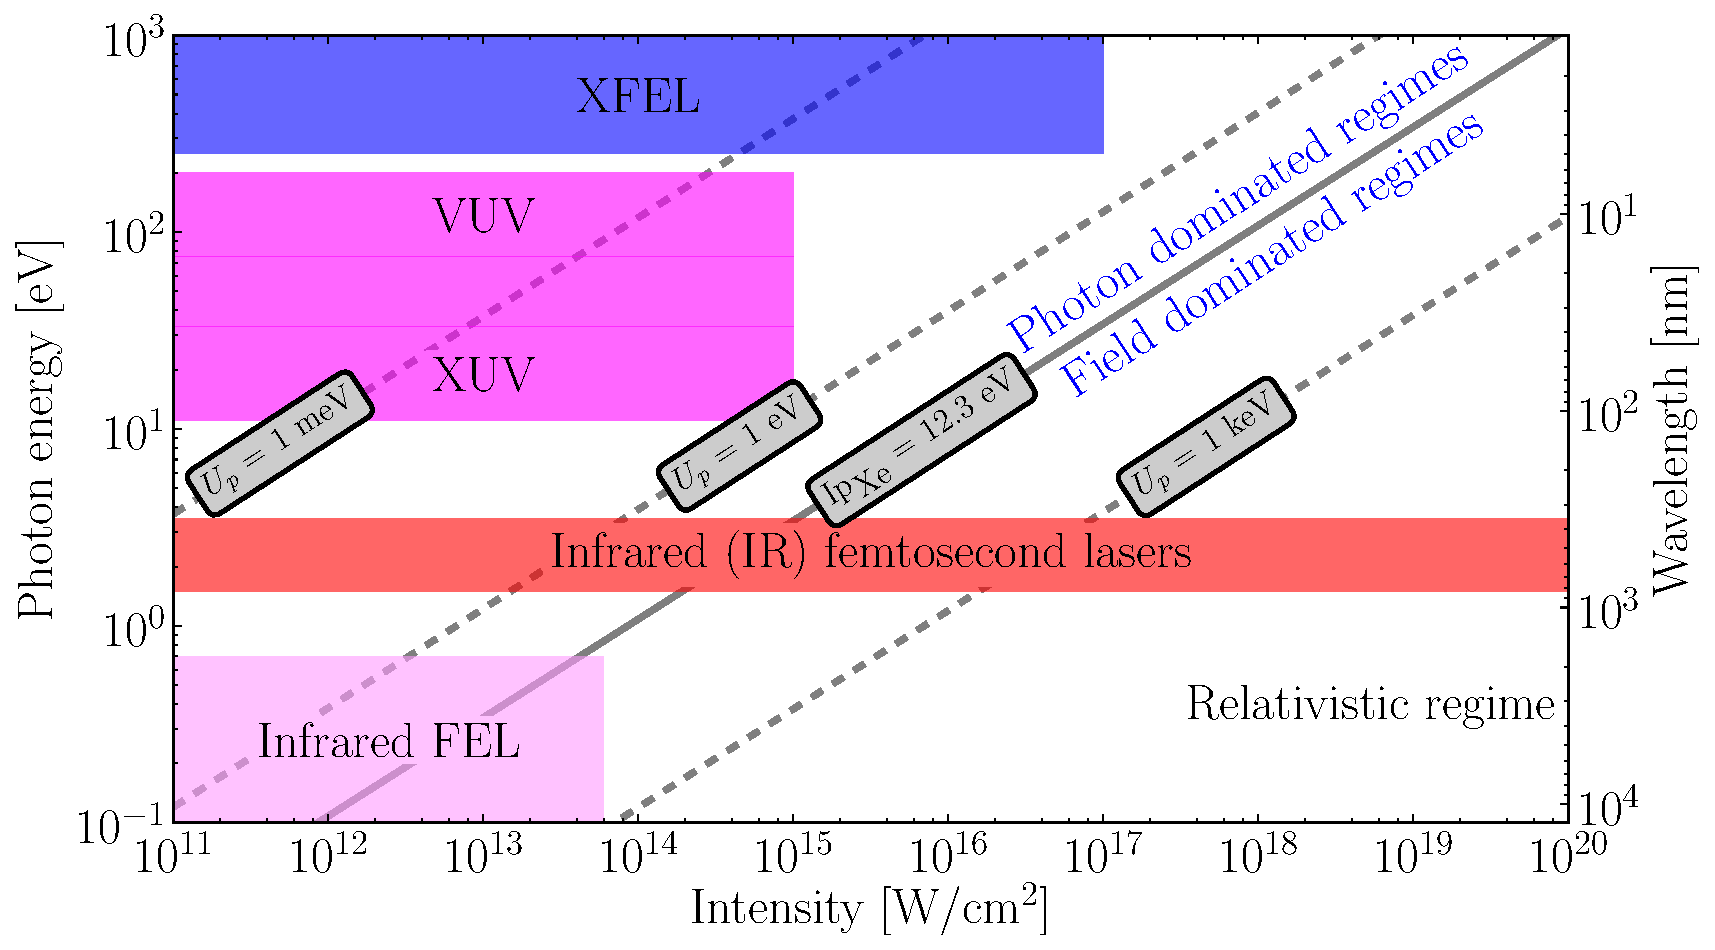
\includegraphics[width=\figurewidth]{figures/regimes}
\caption{Wavelength and intensity regimes. For xenon, the lower right half is dominated
         by field processes and the upper left half by photon processes. Diagonal
         lines represent constant ponderomotive potential $U_p$. The
         demarcation between the two halves occurs when the ponderomotive
         potential equals the ionization potential ($U_p = Ip$).
         Note that the present work concentrates on the VUV and XUV regimes
         where photon processes dominate (at the studied intensities).}
\label{fig:regimes}
\end{figure}

In table \ref{tab:ips} the first ionization energies of the different
rare gas elements used in this thesis (argon and xenon) are shown. As can be
seen from table \ref{tab:ips} and figure \ref{fig:regimes}, xenon and argon can be
single-photon ionized in the VUV regime where photons of 15.76 (for argon)
and 12.13 eV (for xenon) are possible. While xenon's 5p states have the smallest
Ip's, the cross-section for photoionization of the 4d shell is approximately ten
times larger at 13.7 nm (90.5 eV) -- the so called xenon giant 4d
resonance~\cite{Becker1986} -- making ionization of these inner-shells
possible~\cite{Thomas2009,Ackad2013}.
% http://photon-science.desy.de/news__events/research_highlights/archive/flash_excites_giant_atomic_resonance/index_eng.html

\begin{table}
\begin{center}
\begin{tabular}{ccccccc} \hline
 & \mc{3}{c}{Argon} & \mc{3}{c}{Xenon} \\
Z &
Configuration
        & Ip [eV]
                    &$\lambda$ [nm]
                                & Configuration
                                        & Ip [eV]
                                                    & $\lambda$ [nm] \\ \hline
% Used in the code:
% 16.00   & 77.49             & 12.265625 & 101.1 \\
% 32.34   & 38.34             & 21.390625 & 57.96 \\
% 48.68   & 25.47             & 31.296875 & 39.62 \\
% 65.02   & 19.07             & 41.859375 & 29.62 \\
% 81.56   & 15.20             & 55.015625 & 22.54 \\ \hline
%
% Experimental data (from NIST):
% http://physics.nist.gov/PhysRefData/ASD/levels_form.html
0 & 3p$^5$  & 15.7596109& 78.6721   & 5p$^6$& 12.129843 & 102.214 \\
1 & 3p$^4$  & 27.62967  & 44.8736   & 5p$^5$& 20.975    & 56.4 \\
2 & 3p$^3$  & 40.735    & 30.4368   & 5p$^4$& 31.05     & 39.9305 \\
3 & 3p$^2$  & 59.58     & 20.8097   & 5p$^3$& 42.20     & 29.3801 \\
4 & 3p$^1$  & 74.84     & 16.5666   & 5p$^2$& 54.1      & 22.9176\\
5 & 3s$^2$  & 91.290    & 13.5814   & 5p$^1$& 66.703    & 18.5875 \\
6 & 3s$^1$  & 124.41    & 9.96577   & 5s$^2$& 91.6      & 13.5354 \\
7 &  &  &   & 4d$^{10}$ & 105.978   & 11.699 \\
8 &  &  &   & 4d$^{9}$  & 179.84    & 6.89414 \\
9 &  &  &   & 4d$^{8}$  & 202.0     & 6.13783 \\
10 &  &  &   & 4d$^{7}$  & 229.02    & 5.41368 \\
11 &  &  &   & 4d$^{6}$  & 255.0     & 4.86213 \\
12 &  &  &   & 4d$^{5}$  & 280.9     & 4.41382 \\
13 &  &  &   & 4d$^{4}$  & 314.1     & 3.94728 \\
14 &  &  &   & 4d$^{3}$  & 342.9     & 3.61575 \\
15 &  &  &   & 4d$^{2}$  & 374.1     & 3.3142 \\
16 &  &  &   & 4d$^{1}$  & 403.9     & 3.06968 \\ \hline
\end{tabular}
\caption{First few ionization potentials for (atomic) rare gas elements.
         Source: NIST~\cite{NIST}}
\label{tab:ips}
\end{center}
\end{table}

Let us now turn to a more detailed examination of the different mechanisms
present in the different regimes, as well as some regime-independent processes.



\subsubsection{Long wavelength: The IR regime}
\label{section:intro:mechanisms:ir}

Most femtosecond lasers are Ti:sapphire lasers that have a wavelength centred around 800 nm.
This type of laser sparked cluster research. They cover a wide range of
intensity and as such can touch different regimes, from the photon-dominated
at low intensities to the field-dominated at higher intensities,
even going up to levels where relativistic effects cannot be neglected.

Much work was done in the field-dominated (IR) regime over the
years as evidenced by the wide literature on the subject, see for example
ref.~\cite{Fennel2010} or~\cite{Ramunno2008}. The VUV and XUV regime
-- the photon-dominated one -- is much less explored and is thus the main
aspect of the present work. Some effects in the IR are still presented here
for clarity. These processes are dominant in the field-dominated regime (see
figure \ref{fig:regimes}).


\subsubsubsection{Above Threshold Ionization (ATI)}

Above Threshold Ionization (ATI) was one of the first observed effects of
intense laser-matter interaction in 1979~\cite{Agostini1979}.
In ATI, more photons are absorbed by atoms
than are normally required to ionize it. This results in photoelectron spectra
showing peaks at energies much larger than expected separated by the photon
energy. Being a multiphoton process, ATI requires large
intensities~($\gamma \ll 1$)~\cite{Krainov1997,Lewenstein2008}.


\subsubsubsection{Tunnel ionization}

The most striking effect in the IR regime is tunnel ionization~\cite{Niikura2009}.
The Coulomb potential of an atom can be bent enough by the (oscillating) laser
field and the probability of a bound electron tunnelling out becomes significant,
as shown in figure \ref{fig:ionization:tunnel}. Tunnel ionization is also
sometimes called optical field ionization (OFI), or more simply field
ionization, since one can describe the process as the laser field being the source
of the potential bending and ionization.
\lrnote{I made the change to the last sentence, but
am still not happy with it. it's b/c the laser field picture is really only a
semiclassical quantum picture in the length gauge. i will clarify more when we
talk and maybe we can edit it appropriately then.}


% Above Threshold Ionization (ATI) https://en.wikipedia.org/wiki/Above_Threshold_Ionization_%28ATI%29
% Strong Field Approximation (SFI)
% http://massey.dur.ac.uk/resources/cpchirila/
\begin{figure}
 \centering
 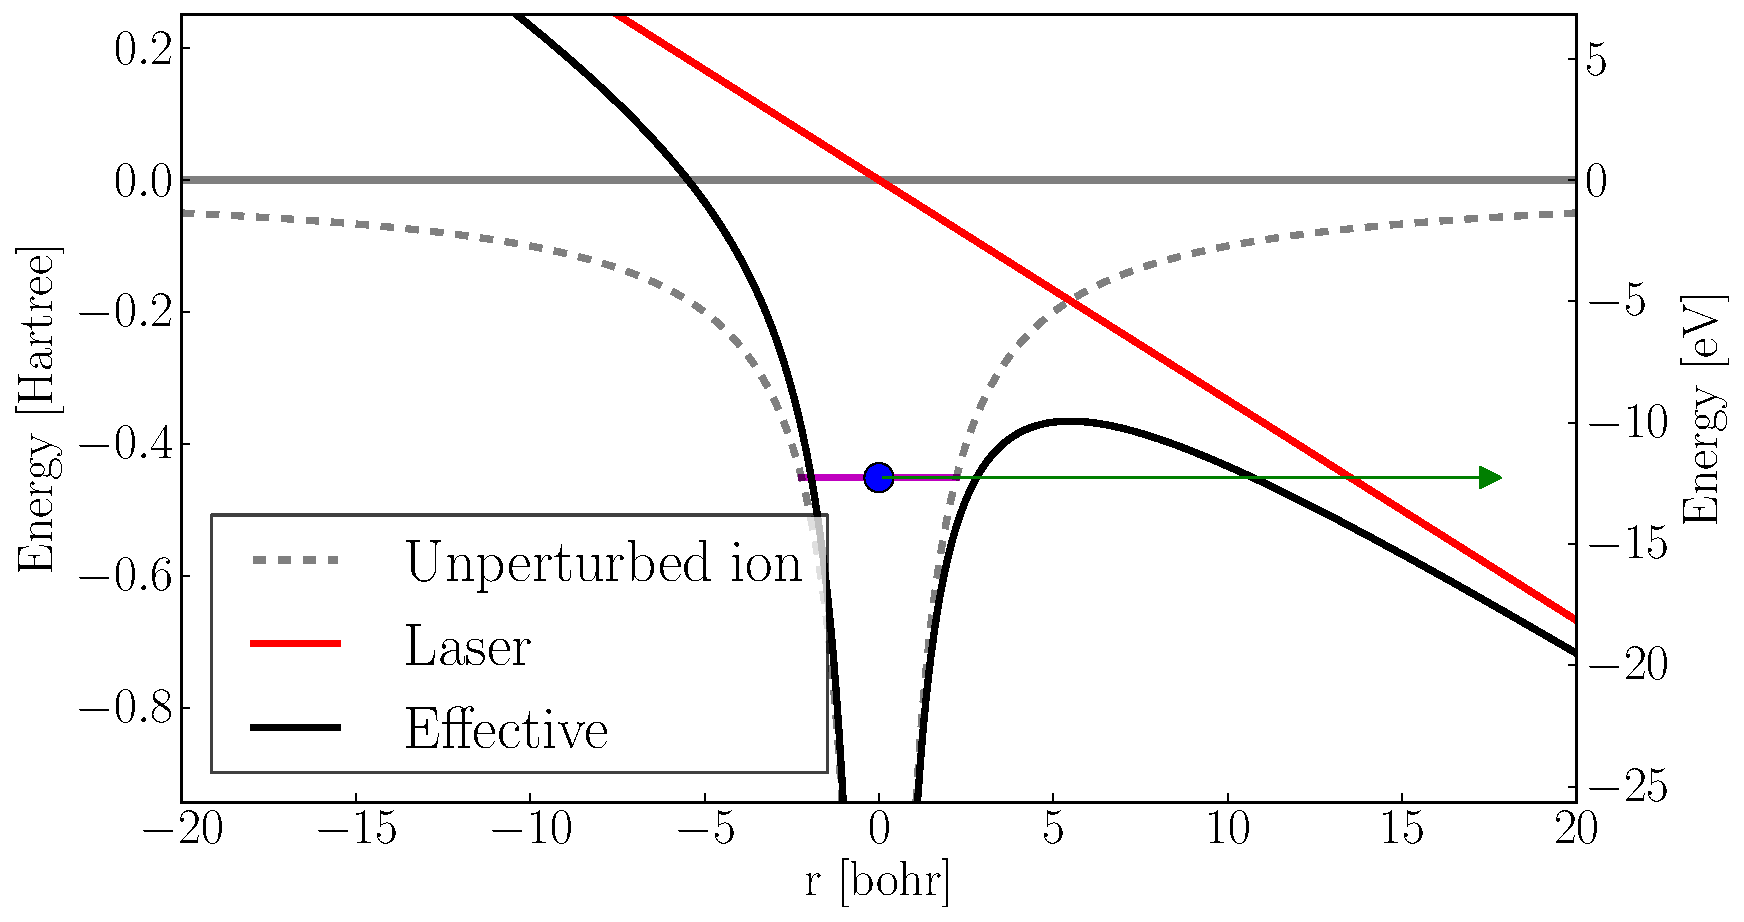
\includegraphics[width=\figurewidth]{figures/ionization_tunnel}
 \caption{\label{fig:ionization:tunnel}Tunnel ionization. The potential
          due to the laser (red) bends the unperturbed ion potential
          (grey dashed). The electron (blue dot) sitting at the unperturbed
          eigenvalue (magenta) now has a probability to tunnel through the total
          potential barrier (black line). The laser frequency must be small
          enough for the probability to be non-negligible (large wavelength)
          and intensity large enough ($\gamma \ll 1$).}
\end{figure}

Tunnel ionization is at the heart of High Harmonic Generation (HHG) and
attosecond science~\cite{Fennel2010}. A laser pulse, normally in the IR regime,
bends the atomic potential felt by bound electrons, allowing them to tunnel
out. They are then accelerated in the laser field where they gain energy.
As the laser field changes direction within a laser cycle, electrons are forced
back onto their parent ion where they can
recombine and emit high energy photons. The emission spectra,
containing only odd harmonics, shows an intensity decrease as a function of
harmonic number, followed by a plateau and a cutoff. Since the description
of the phenomena in 1993~\cite{Corkum1993}, HHG studies expanded into its own
sub-field. For example, Murphy \textit{et al.} used the 21st harmonic of a
800 nm Ti:sapphire to ionize xenon clusters~\cite{Murphy2008a,Murphy2008b}
with these new 32.6 eV (38 nm) photons.
For more details on HHG see references~\cite{Levesque2006}
and~\cite{Lewenstein2008}.
\lrnote[noinline,margin]{you should be prepared to answer "why only odd harmonics?"}


\subsubsubsection{Inverse Bremsstrahlung Heating}

Once electrons are created in the IR regime they can continue to absorb energy
from the laser.
Inverse Bremsstrahlung Heating (IBH) is the inverse process of Bremsstrahlung
where an electron emits a photon when deflected, either by a heavier ion in the
case of plasma, or by magnetic fields in the case of synchrotrons. IBH is thus
the absorption of photons accelerating the electrons~\cite{Schlessinger1979}.

For large frequencies, the quiver amplitude of equation \eqref{eqn:quiver} is
small; the electric field oscillates
too rapidly for the electrons to gain significant acceleration.
But for smaller frequencies (larger wavelengths), the quiver amplitude can
be significant. In the case of IR, electrons can be pushed outside the cluster
and back in; at $\ten{3}{16}$~W/cm$^2$ and 800~nm, the quiver
amplitude is $x_q \approx 500 a_0$, where $a_0$ is the Bohr
radius~\cite{Georgescu2007}, while a Xe$_{1,415}$ cluster is~115~$a_0$.

The linear momentum gained by electrons in the laser field is then redistributed
as thermal energy by collisions and scattering on heavier ions.
IBH plays an important role in the IR regime where the laser field easily
drives the electrons through the cluster~\cite{Fennel2010}.

% The energy $E$ change rate over time due to IBH is given~\cite{Fennel2010} by:
% The IBH rate is given~\cite{Fennel2010} by:
The rate of change of energy $E$ over time due to IBH (per electron) is
given~\cite{Fennel2010} by:
\begin{align}
\left< \dt{E} \right> & = 2 U_p \frac{\tau \omega^2}{\tau^2 \omega^2 + 1},
\end{align}
where $\tau$ is the inverse of the electron-ion collision frequency, $\omega$ the
angular frequency of the laser and $U_p$ the ponderomotive potential.

\fxnote{According to Bostedt2010\cite[page 3]{Bostedt2010}, IBH scales as
$\lambda^{8/3}$ and cites Krainov2000~\cite{Krainov2000} and
Krainov2002~\cite{Krainov2002}}
% ? can you explain the problem to me when we talk next?

\subsubsection{Shorter wavelengths: Into the VUV and XUV regime}
\label{section:intro:mechanisms:vuv}

% http://www.laserfocusworld.com/blogs/what-the-hecht/2012/05/euv-xuv-acronym.html
% http://www.spacewx.com/Docs/ISO_PRF_21348_e_review.pdf
% http://www.iso.org/iso/home/store/catalogue_tc/catalogue_detail.htm?csnumber=39911

With new FEL facilities, high laser intensities can be reached at
lower wavelength (and thus larger photon energy) than traditional
femtosecond lasers. \textit{Vacuum ultraviolet} (VUV) radiation, ranging from 200 to
10~nm (6.2 to 124~eV), is normally absorbed by the atmosphere. Its study
requires vacuum chambers (hence the name) or a pure nitrogen propagation medium.
At short wavelengths, the photons can start to ionize inner shell electrons. In
that case, the term \textit{extreme ultraviolet} (XUV, or EUV) is used. XUV wavelengths
range from 121~nm (hydrogen's Lyman alpha line, 10.25 eV) to 10~nm (124~eV).
As the two regimes have overlapping wavelengths, they are often used
interchangeably but XUV is generally used with wavelengths where no
material is known to be transparent~\cite{Laane2009}. Note that in other fields,
XUV can be used to describe soft X-rays~\cite{Eichmeier2008,iso21348}

At relatively low intensity (less than 10$^{14}$~W/cm$^2$
~\cite{Ramunno2008}), in the photon-dominated regime, atoms and ions
can be ionized by photon absorption. If the photon energy is superior to the
electron's binding energy (see table \ref{tab:ips} for numerical values) single
photon ionization will be the dominant energy transfer mechanism.

While not as strong as in the IR regime, IBH is still important in the
VUV~\cite{Krainov2000} up to 62 nm~\cite{Georgescu2007}.


\subsubsubsection{Photon absorption}

Initially described by Einstein as the photoelectric effect, a bound electron
absorbs a photon from the laser and is promoted to the continuum where it is
free to leave its parent ion. Figure~\ref{fig:ionization:single} shows a
schematic of the mechanism. For example, the first energy level of atomic
xenon is at -12.27 eV, requiring a photon wavelength equal or shorter than
101.1 nm for ionization.


\begin{figure}
 \centering
 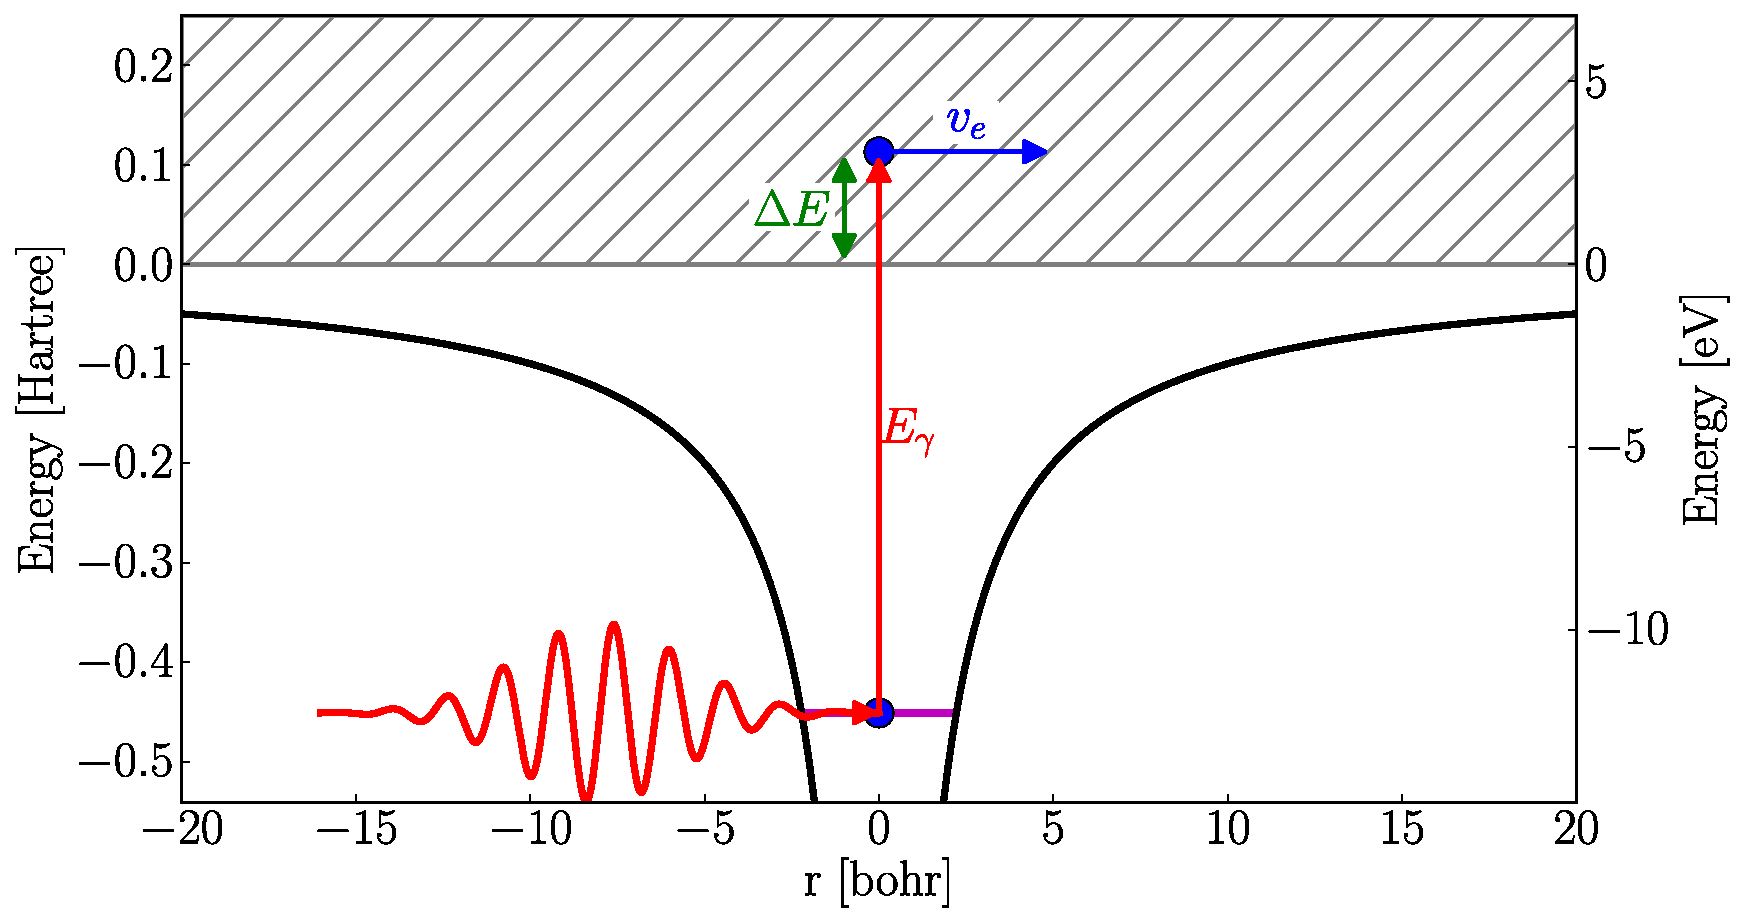
\includegraphics[width=\figurewidth]{figures/ionization_single}
 \caption{Single photon ionization for the atomic, isolated model. A photon
          (red) is absorbed by a bound electron (blue) which is promoted to
          the continuum. The remaining energy $\Delta E$ between the photon's
          and the Ip results in electron's kinetic energy $K_e$.
          Chapter \ref{section:tools} describes the cluster environment
          influence.}
 \label{fig:ionization:single}
\end{figure}

If the photon energy exceeds the electron's binding energy, the difference in energy
will be transferred as extra kinetic energy in the
resulting photoelectron. Thus, it can be used to sample the states in the
target by measuring the photoelectron energy spectrum~\cite{Fennel2010}.

However, if the photon energy is less than the binding energy, then a single
photon cannot ionize an atom. But if the intensity is large enough, the
photon density will be sufficient that many photons can be absorbed during a
small time interval.
This effect is called multiple-photon ionization (MPI, not to
be confused with the Message Passing Interface used in parallel programming) and
is a non-linear process. The ionization rate of $\nu$-photon MPI is given
by~\cite{Fennel2010}:
\begin{align}
\Gamma_{\nu} = \sigma_{\nu} I^{\nu}.
\label{eqn:ionization:rate:mpi}
\end{align}
Being a nonlinear process, multi photon ionization becomes significant at higher
intensities than single photon ionization. But being photon processes, both are
superseded by tunnel ionization at even higher intensities (or when
$\gamma~\gg~1$).


% \clearpage
\subsubsubsection{Auger effect}

At even shorter wavelength, the photon energy might be large enough to not only
ionize the highest energy electron but also some inner-shell electrons.
When such an inner shell electron gets ionized, it leaves a hole; the atom is
thus in an excited state. An outer shell electron will then transition by
\textit{Auger decay} to the hole. The transition energy is used by a third
electron (the Auger electron) to leave the ion, leaving the latter
doubly-ionized. Figure \ref{fig:auger} shows a diagram of the process.

\begin{figure}
 \centering
    \begin{subfigure}[t]{0.45\columnwidth}
        \centering
        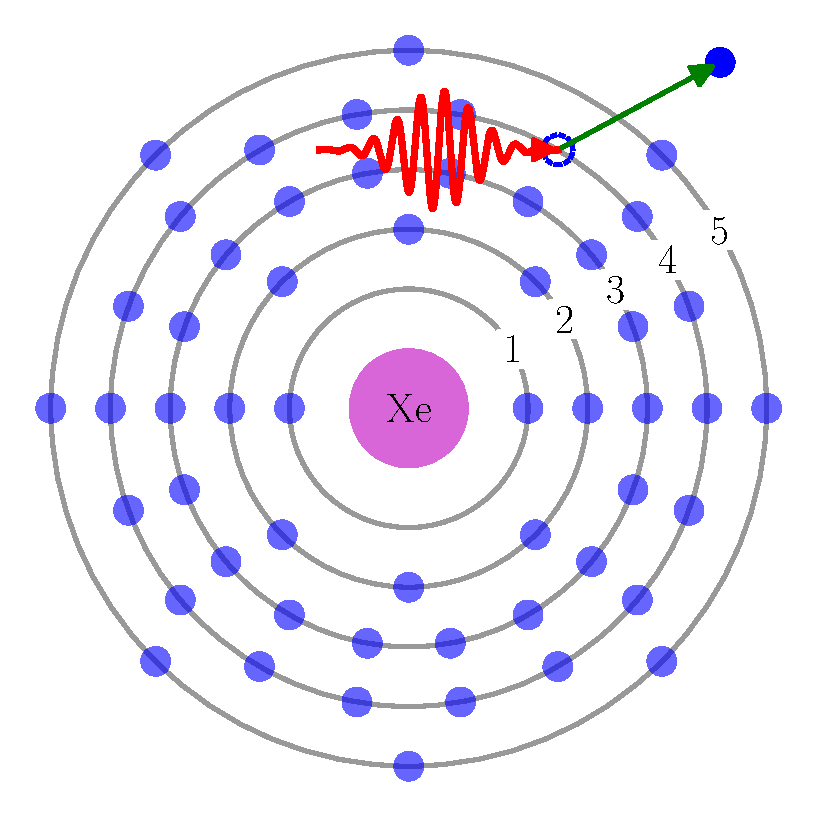
\includegraphics[width=\textwidth]{figures/auger_step_1}
        \caption{Step 1: An xenon 4d inner shell electron absorbs a high
                 energetic photon and leaves the atom.}
        \label{fig:auger:1}
    \end{subfigure}
    \hspace{20pt}
    \begin{subfigure}[t]{0.45\columnwidth}
        \centering
        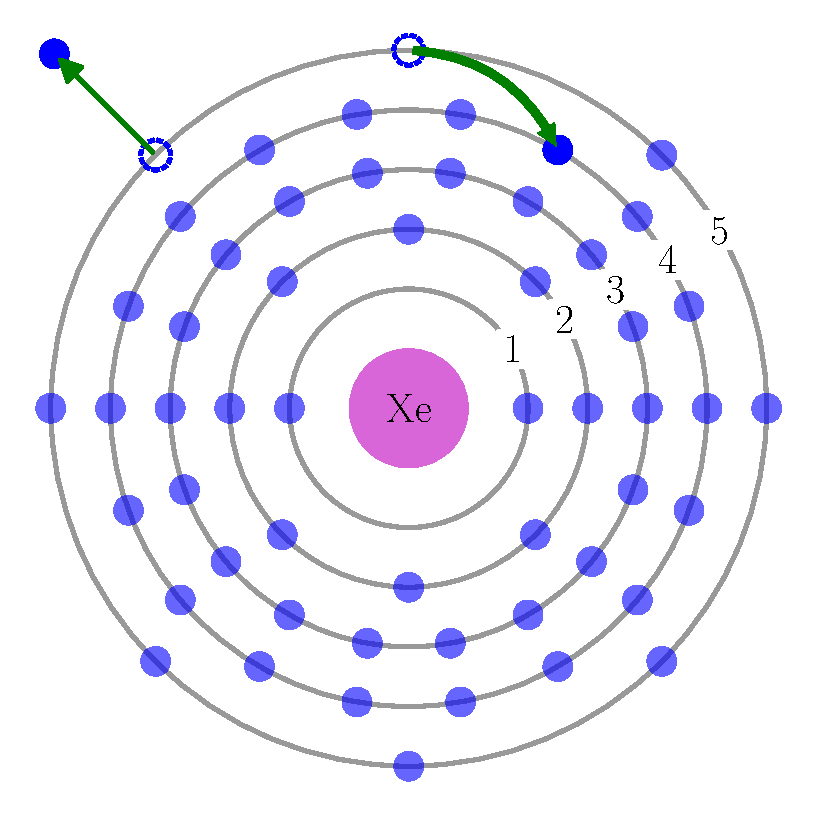
\includegraphics[width=\textwidth]{figures/auger_step_2}
        \caption{Step 2: An outer shell electron decays into the created hole,
                 transferring the energy difference between the two states to a
                 third electron which is ejected (the Auger electron).}
        \label{fig:auger:2}
    \end{subfigure}
        \caption{\label{fig:auger}Auger ionization of a xenon 4d electron by a
                 high energetic X-ray photon. Xenon's 54 electrons are shown
                 as blue dots with the distance to the core representing their
                 principal quantum numbers $n$.}
\end{figure}

To access core electrons, photons must be highly energetic, as usually found in X-rays.
While not the focus of the present work, an interesting aspect is that xenon
atoms have a giant resonance of the (inner-shell) 4d state; the cross-section of
photoionization of the 4d electron is ten times larger than the
one of valence  electrons at 13.7 nm wavelength~(90.5~eV)~\cite{Becker1986}.
This process was included in the model for a comparison with a 2009 experiment
by Thomas \textit{et al.}~\cite{Thomas2009} on xenon clusters at FLASH-DESY.
The German group saw clusters becoming nanoplasmas from which the outer shell
ions undergo Coulomb explosion while the relatively neutral core expands
hydrodynamically. These results could be reproduced by our model as shown in a recently
published article entitled ``Recombination effects in soft-x-ray cluster
interactions at the xenon giant resonance'', published in May 2013 in
\textit{New Journal of Physics}~\cite{Ackad2013} and included in chapter
\ref{section:papers:recomb}.

% ******************************************************************************
\subsubsection{Regime independent processes}
\label{section:intro:mechanisms:noregime}

Once electrons are created in the cluster, other mechanisms appear. During
impact ionization a first electron collides with an atom and, if it has enough
kinetic energy, will transfer a portion of it to a bound electron, promoting it
to the continuum. Figure \ref{fig:ionization:impact} shows the energy diagram
of the process.

\begin{figure}
 \centering
 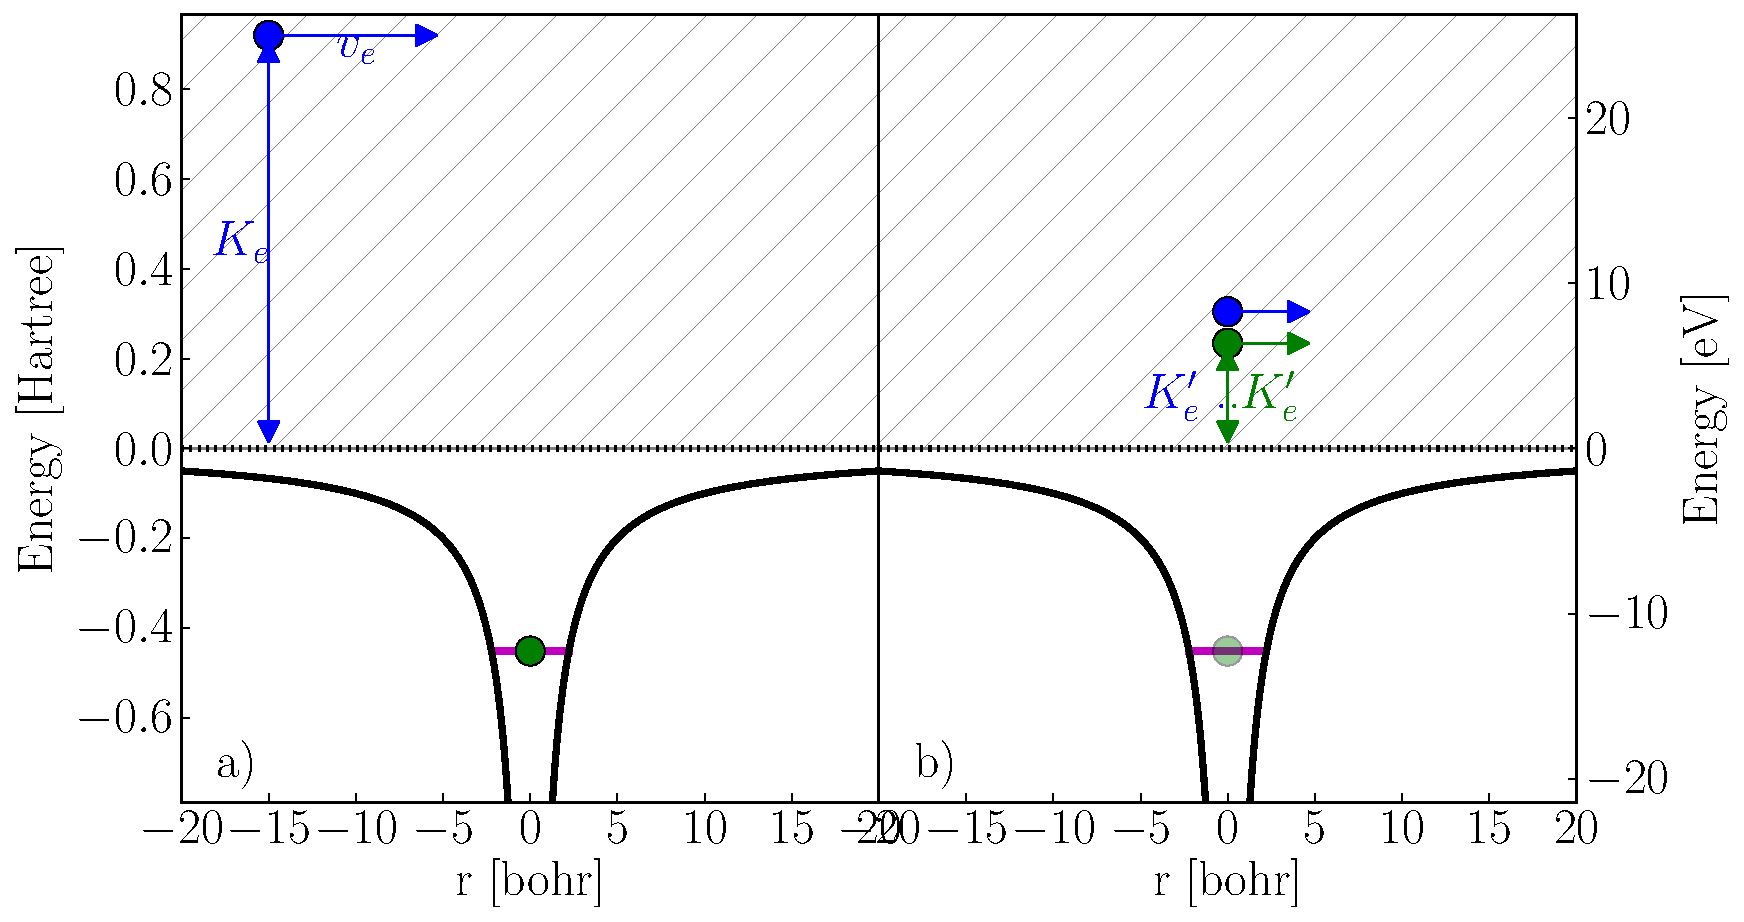
\includegraphics[width=\figurewidth]{figures/ionization_impact}
 \caption{Impact ionization. The colliding electron (blue dot) gives a portion
          of its energy to a bound electron (green dot), promoting it to the
          continuum.}
 \label{fig:ionization:impact}
\end{figure}

Impact ionization can be modelled through cross-sections. These
cross-sections are normally obtained from the semi-empirical Lotz
formula~\cite{Lotz1967}:
\begin{align}
\sigma & = \sum_{i}^{N} a_i q_i \frac{\ln{\pa{E/\textrm{Ip}_i}}}{E \textrm{Ip}_i} \pa{1 - b_i
\ex{-c_i \pa{E/\textrm{Ip}_i - 1}}},
\label{eqn:impact:ionization:lotz}
\end{align}
where Ip$_i$ is the ionization potential of the $i^{\textrm{th}}$ shell and $E$
the impacting electron's kinetic energy \textit{at infinity} (or above threshold).

\subsubsection{New regime, new processes}
\label{section:intro:mechanisms:new},

By going to shorter wavelengths, FEL installations allowed experiments at high
intensities in the VUV and XUV regime. These experiments saw surprisingly
high charge states resulting from the cluster
explosion~\cite{Wabnitz2002,Bostedt2010}. For example, Wabnitz \textit{et al.}
saw, at FEL-DESY, Xe$^{4+}$ when Xe$_{80}$ clusters were irradiated with 98 nm,
100 fs FEL pulses of, what was thought at the time, $\ten{2}{13}$~W/cm$^2$
intensity. For larger clusters (Xe$_{30,000}$), xenon ions up to
Xe$^{8+}$ were observed. This was surprising as the 98~nm
photons (12.7 eV) could only ionize neutral xenon to Xe$^{1+}$ by themselves;
data showed that up to 30 photons were absorbed per atom for the largest
clusters. Using a different source of photons and at a different wavelength
(21st harmonic of an 800 nm Ti:sapphire, XUV: 32.6 eV, 38 nm),
Murphy \textit{et al.} observed the same pattern of high charge states in xenon
clusters~\cite{Murphy2008a,Murphy2008b}.

Such high charge states could not be explained by the previous processes only.
New mechanisms were thus proposed to explain these surprising results.
The four main models proposed throughout the years are covered next.


\subsubsubsection{Atomic potentials}

First, Santra \& Greene proposed using \textit{atomic potentials} instead of
the Coulomb potential in a rate equation model (with infinite spatial
extension and
constant density) as seen on figure \ref{fig:heating:atomic_pot}.
The atomic nucleus is normally shielded by bound electrons but inside the
electronic cloud the shielding disappears and the nucleus potential is more
important. If an impacting electron can get close enough to the core, it will
feel the unshielded potential.
In reference~\cite{Greene2003}, Santra \& Greene used an approximated form for
the atomic potential, fitting one parameter with the first ionization potential.
A later~\cite{Walters2006} publication used a
potential shape generated by the code written by Herman and
Skillman~\cite{HS1963} (HS) to describe a more realistic
potential, based on a
Hartree-Fock formulation. Using these atomic potentials, they saw Xe$^{3+}$,
Xe$^{5+}$ and Xe$^{7+}$ for intensities of $\ten{1.4}{12}$, $\ten{1.4}{13}$ and
$\ten{7.3}{13}$~W/cm$^2$ respectively for Xe$_{1,500}$ clusters, similarly to
what was seen in at FEL-DESY.

\newpage
\subsubsubsection{Barrier suppression}

Another model proposed by Siedschlag and Rost~\cite{Siedschlag2004} in 2004 was
the barrier suppression in single photon absorption which is shown on figure
\ref{fig:heating:barrier}. Due to the proximity
of neighbours, the potential barrier between them is lowered and
a photo-transition to the continuum becomes possible, even with a single photon.

\lrnote{nic, did we ever talk about the downsides of the rost model?}

\subsubsubsection{Many-Body Recombination}

\textit{Many-Body Recombination} (MBR) was proposed in 2005~\cite{Jungreuthmayer2005}
as a simple mechanism to explain the high charge states seen in the
experiments at FEL-DESY. In a strongly coupled plasma, electrons can recombine
easily to a high excited
state after collisions with numerous bodies. Later, these newly bound electrons can
absorb a new photon from the laser field for another transition to the
continuum -- see figure \ref{fig:heating:mbr}.
Because MBR is much more efficient than three-body
recombination (due to the large density of charged particles), much more
photons are absorbed this way. It was also shown that MBR deposited more energy
in the clusters than traditional IBH.
The method's simplicity
lies in the fact that in a classical MD simulation, MBR is automatically
included without extra implementation as the high excited states have energies
which are close to each other and can thus be treated classically.
Jungreuthmayer \textit{et al.} were able
to see Xe$^{3+}$, Xe$^{5+}$ and Xe$^{7+}$ for intensities of $\ten{1.5}{12}$,
$\ten{1.5}{13}$ and $\ten{7}{13}$~W/cm$^2$ respectively when simulating
Xe$_{1,000}$ clusters.

\begin{figure}
 \centering
    \begin{subfigure}{0.48\columnwidth}
        \centering
        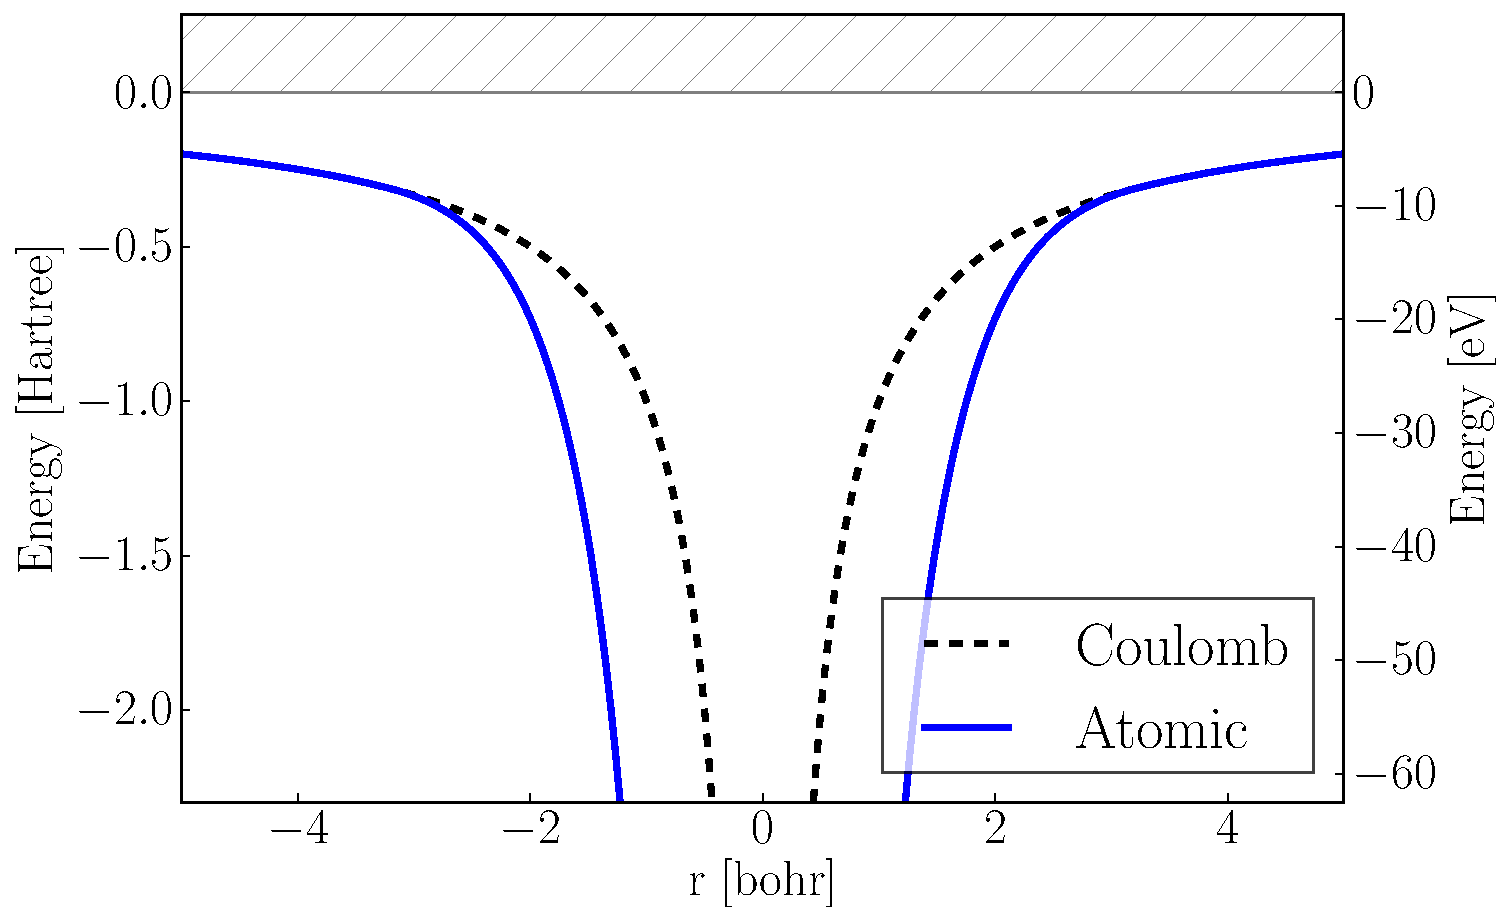
\includegraphics[width=\textwidth]{figures/heating_atomic_potential}
        \caption{Atomic potential (blue line) drops faster than Coulomb one
                (black dashed line), allowing more energy absorption through
                IBH.\\}
        \label{fig:heating:atomic_pot}
    \end{subfigure}
%
    \begin{subfigure}{0.48\columnwidth}
        \centering
        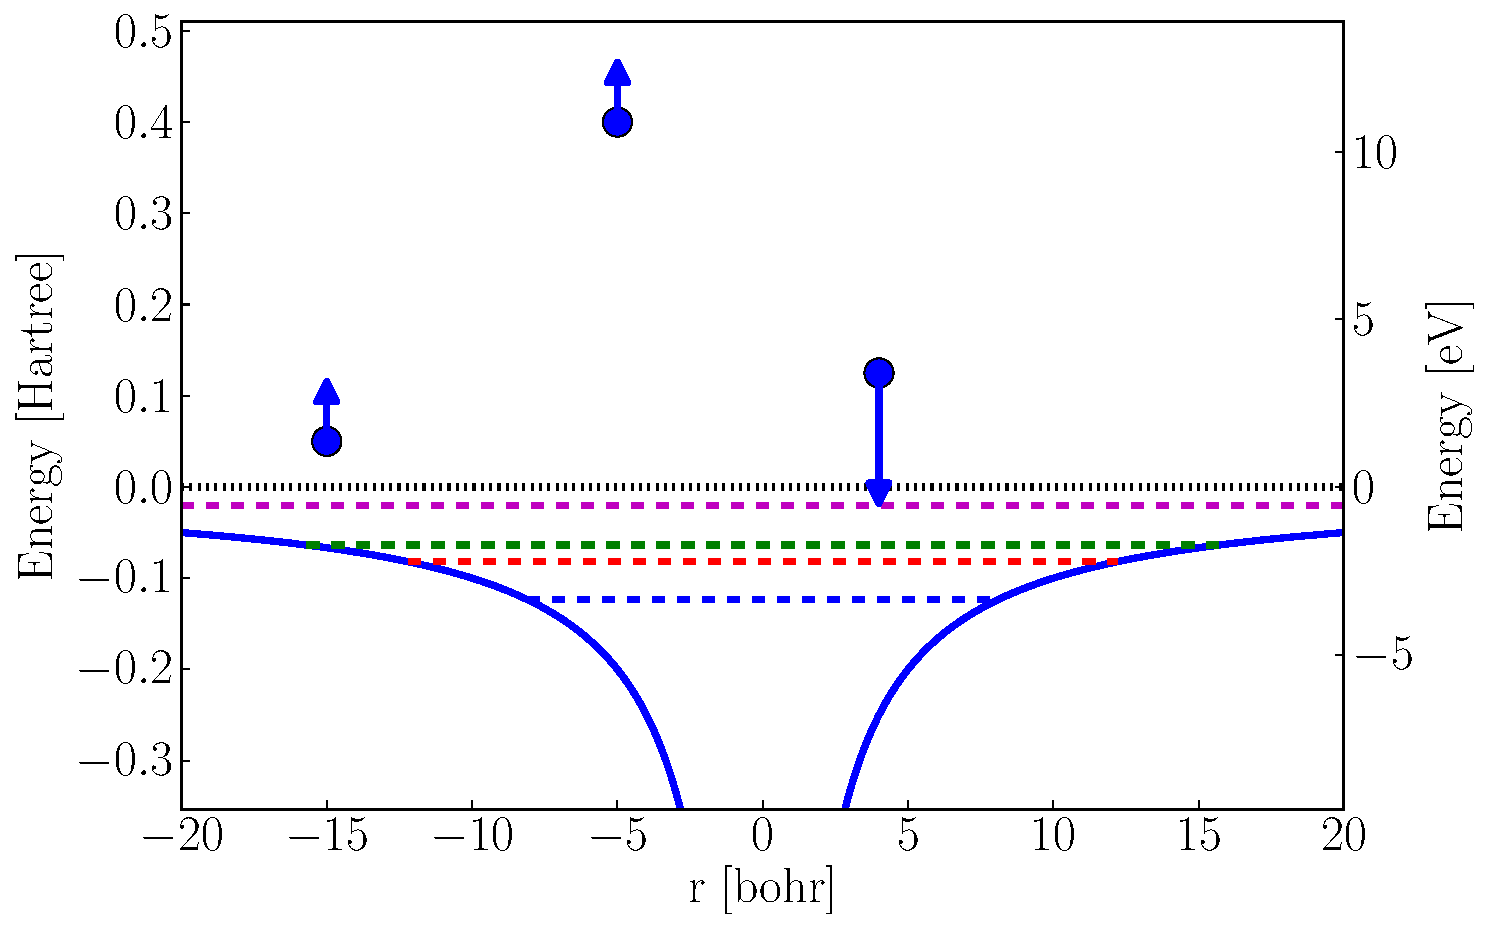
\includegraphics[width=\textwidth]{figures/heating_mbr}
        \caption{MBR: energy exchange between free electrons during collisions
                 makes one recombine to a highly excited state where it can
                 reabsorb a new photon from the laser field.}
        \label{fig:heating:mbr}
    \end{subfigure}
\\
    \begin{subfigure}{\figurewidth}
        \centering
        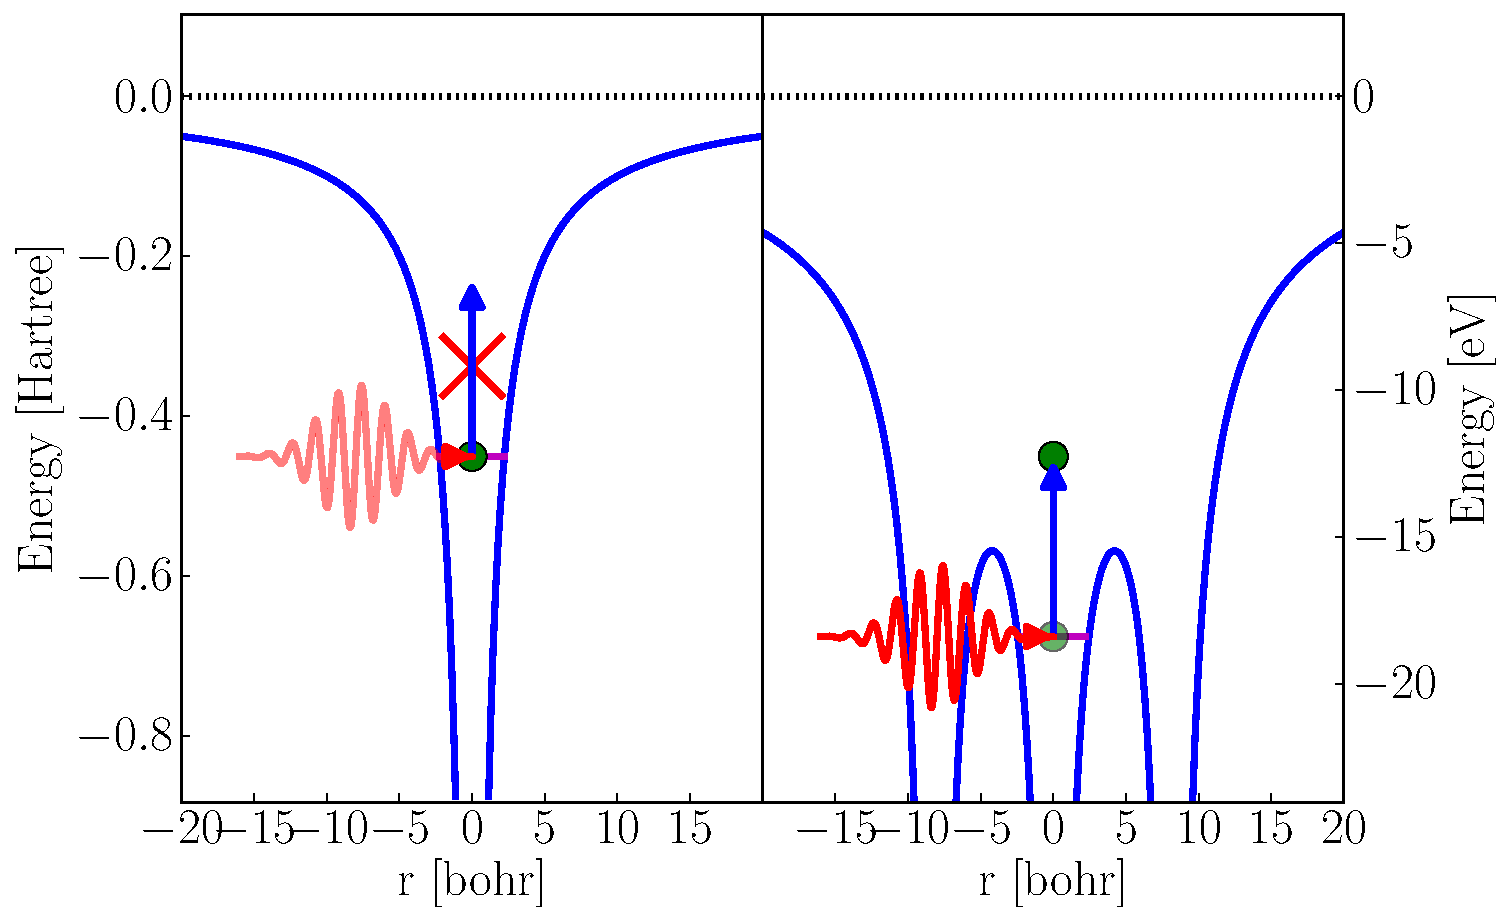
\includegraphics[width=\textwidth]{figures/heating_barrier_sup}
        \caption{Barrier suppression between ions in a cluster environment allows
                 a single photon to ionize deeper levels (right), not accessible
                 with a single atom (left).}
        \label{fig:heating:barrier}
    \end{subfigure}
 \caption{More heating mechanisms}
 \label{fig:heating}
\end{figure}

